\documentclass{bbawslides}

\usepackage[TS1, T1]{fontenc}
\usepackage{ifthen}

\usepackage[a4paper]{hyperref}
\rotateheaderstrue	%%-- otherwise seminar does strange things
\usepackage{url}

\usepackage[ngerman]{babel}
\usepackage[babel]{csquotes}
\usepackage[autoplay]{animate}
\usepackage{graphicx}
\usepackage{numprint}
\npthousandsep{~}\npthousandthpartsep{}\npdecimalsign{,}

\DeclareTextSymbol{\textlongs}{TS1}{115} 
\DeclareTextSymbolDefault{\textlongs}{TS1}


\begin{document}
\providecommand{\Title}{}


\begin{bbawtitle}[Perspektiven der automatischen Texterfassung als Grundlage
wissenschaftlicher Editionen]
  \vspace*{0.5em}%
  \textcolor{bbawred}{\bf am Beispiel der Brief- und Schriftenausgabe\\der \textsc{Bernd Alois Zimmermann}-Gesamtausgabe}\\[4ex]
  Matthias Boenig, Hemma Jäger, Matthias Pasdzierny, Kay-Michael Würzner\\[-.25em]%
  \textcolor{urlColor}{\texttt{{\small \{boenig|hemma.jaeger|pasdzierny|wuerzner\}@bbaw.de}}}
  \\[1.5em]
  {\scriptsize{%
    Geisteswissenschaftliche Forschungsdaten.\\Methoden zur digitalen Erfassung, Aufbereitung und Präsentation\\%
    19. Oktober 2017\\%
  }}
\end{bbawtitle}
\slideStyleFrame

\renewcommand{\footerText}{\tiny 19. Oktober 2017, Workshop AG eHumanities}

%----------------------------------------------------------------------------------------------
% Outline
%----------------------------------------------------------------------------------------------
\begin{bbawslide}{Übersicht}
  \vspace*{7mm}%
  \centerslidestrue%
  \begin{itemize}
    \item Einleitung
    \begin{itemize}\small
      \item die \textsc{Bernd Alois Zimmermann}-Gesamtausgabe
      \item automatische Texterfassung
      \item Motivation
    \end{itemize}
    \item Workflowbeschreibung
    \begin{itemize}\small
      \item Bildvorverarbeitung
      \item Layoutanalyse
      \item Zeichenerkennung
      \item Textbearbeitung
    \end{itemize}
    \item Perspektiven
    \begin{itemize}\small
      \item Volltextverbesserung
      \item OCR-D
      \item Editionsunterstützung
    \end{itemize}
  \end{itemize}
\end{bbawslide}

\begin{bbawslide}{Die \textsc{Bernd Alois Zimmermann}-Gesamtausgabe}
  \vspace*{7mm}%
  \centerslidestrue%
  \textbf{Matthias}
  \begin{itemize}
    \item
  \end{itemize}
\end{bbawslide}

\begin{bbawslide}{Die \textsc{Bernd Alois Zimmermann}-Gesamtausgabe}
  \vspace*{7mm}%
  \centerslidestrue%
  \textbf{Matthias}
  \begin{itemize}
    \item
  \end{itemize}
\end{bbawslide}

\begin{bbawpart}{\Large\bf Einleitung}
\end{bbawpart}

\begin{bbawslide}{Automatische Texterfassung}
  \vspace*{7mm}%
  \hspace*{-2.5em}%
  \centerslidestrue%
  \begin{tabular}{lc}
    \begin{minipage}{0.65\textwidth}
      \begin{mitemize}
        \item Huge amount of text sources not available in \emph{digital} form
        \begin{mitemize}\small
          \item Historical books, newspapers, and papers from the printing era
          \item Hand-written manuscripts and letters
        \end{mitemize}
        \item Conservation by scanning or photographing
        \begin{mitemize}\small
          \item Images but \textbf{no text data}
          \item[\textcolor{bbawred}{$\Rightarrow$}] Text retrieval or quantitative analyses impossible
        \end{mitemize}
        \item Automatic capturing of \textbf{text} within images
        \item Automatic capturing of \textbf{layout} within images (aka.~\textbf{O}ptical \textbf{L}ayout \textbf{R}ecognition)
      \end{mitemize}
    \end{minipage}
    &
    \begin{minipage}{0.4\textwidth}
        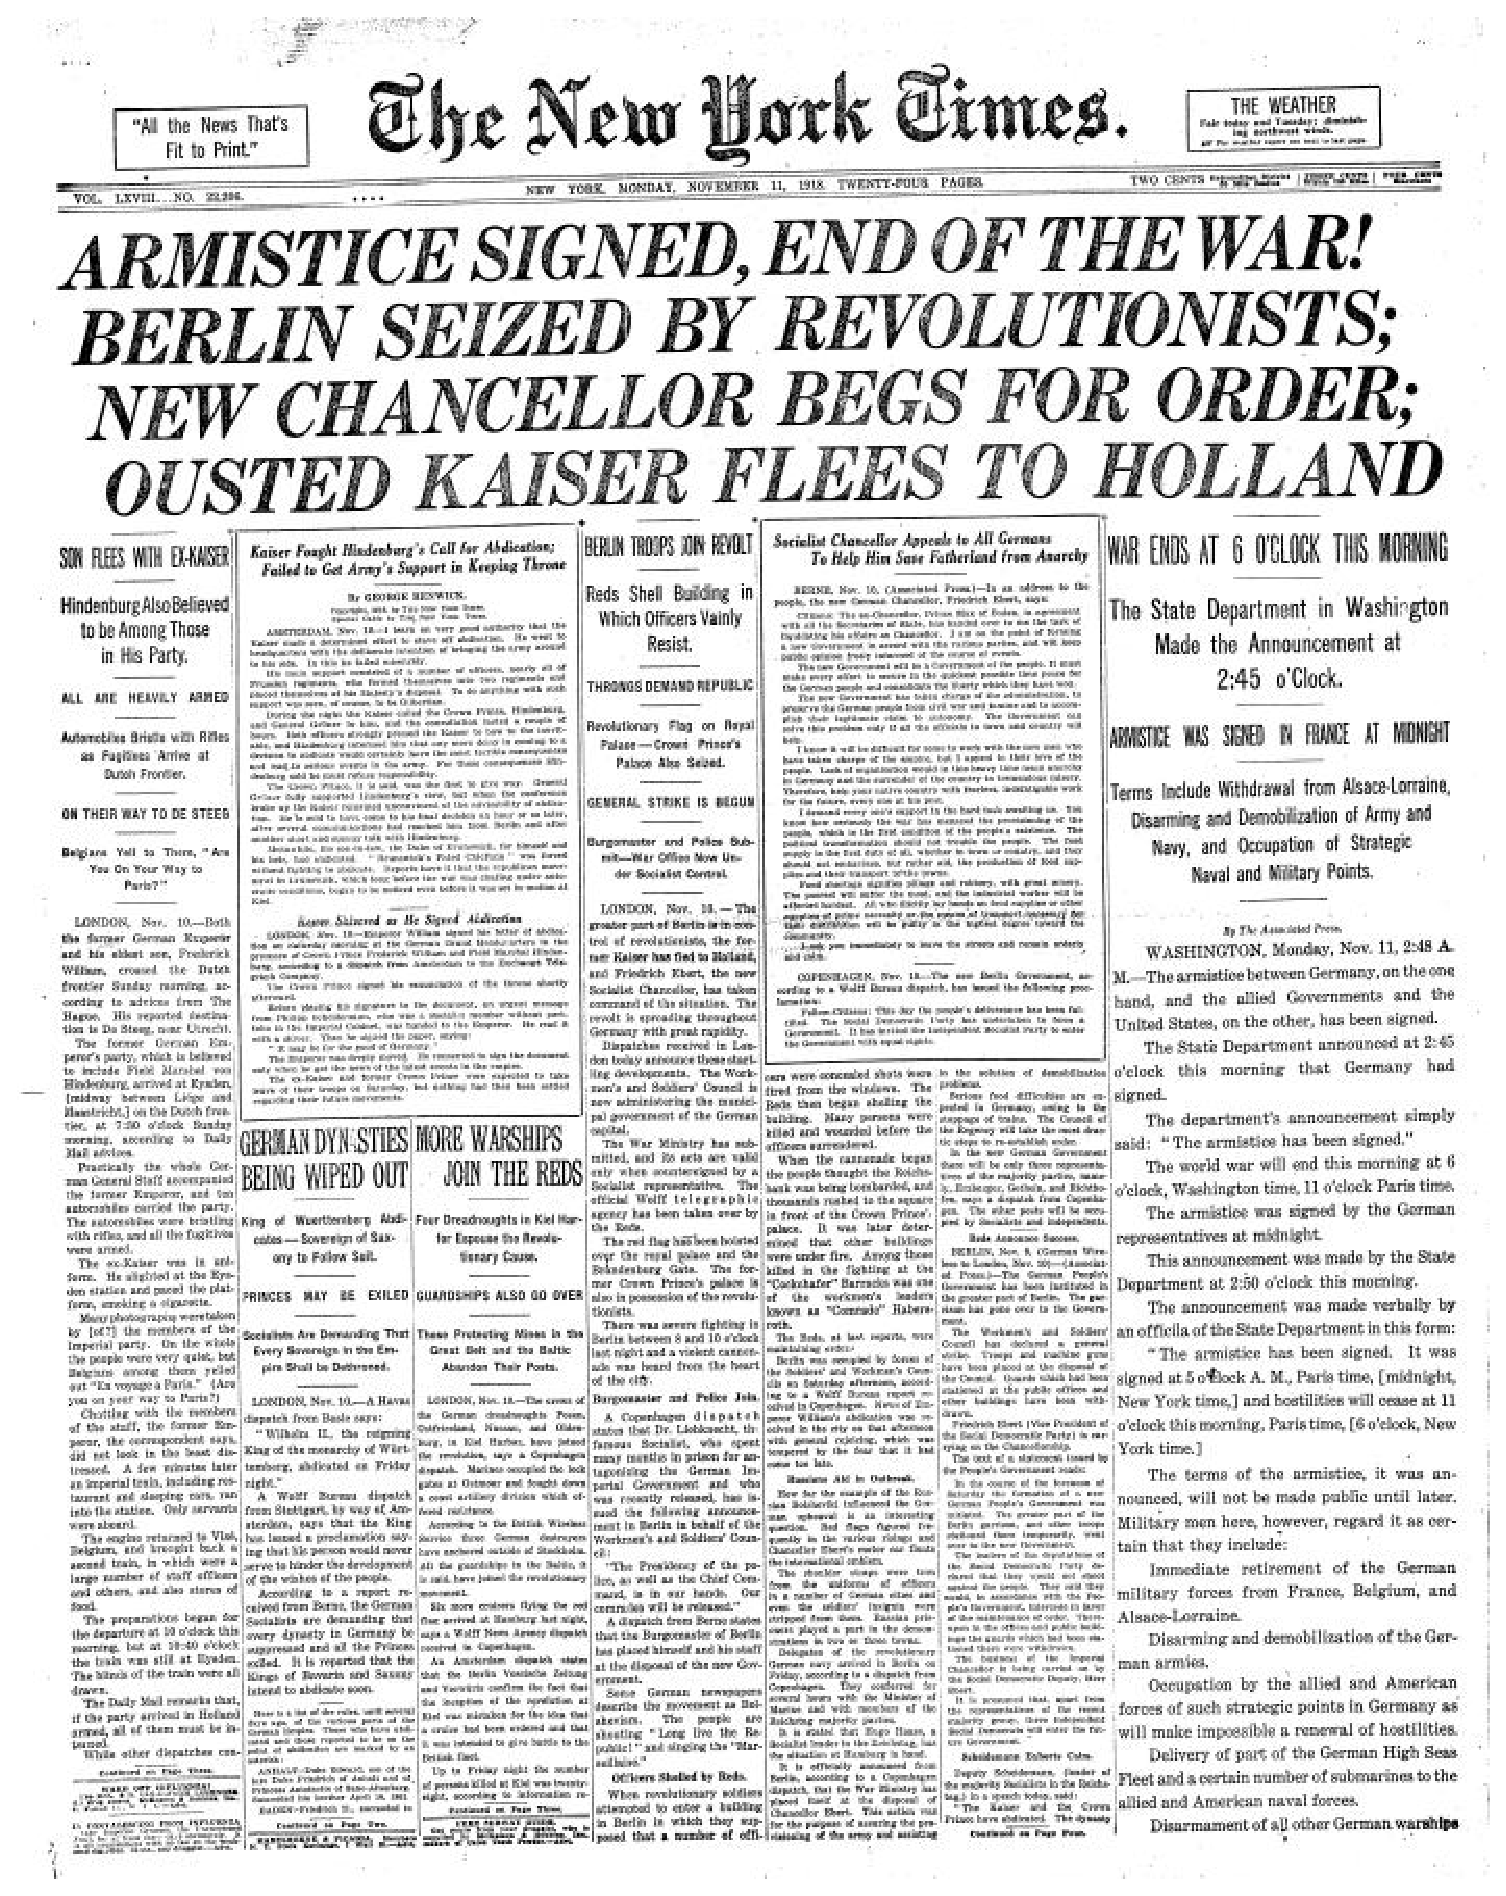
\epsfig{file=figures/times.eps,width=\textwidth}
    \end{minipage}
  \end{tabular}
\end{bbawslide}

\begin{bbawpart}{\Large\bf Workflowbeschreibung}
\end{bbawpart}

\begin{bbawslide}{Übersicht}
  \vspace*{7mm}%
  \centerslidestrue%
  \begin{itemize}
    \item
  \end{itemize}
\end{bbawslide}

\begin{bbawslide}{Bildvorverarbeitung}
  \vspace*{7mm}%
  \centerslidestrue%
  \begin{itemize}
    \item Prozesse zur bestmöglichen Vorbereitung der Digitalisate für OLR und OCR
    \begin{itemize}\small
      \item \textbf{Cropping:} Beschneidung des Digitalisats auf den Druckbereich
      \item \textbf{Deskewing:} Rotation des Digitalisats zur Begradigung von Schrägstellungen
      \item \textbf{Binarization:} Binäre Kodierung der Pixel (bedruckte Bereiche schwarz, nicht-bedruckte Bereiche weiß)
      \item \textbf{Despeckling:} Entfernung von Bildartefakten (Verschmutzungen, sichtbare Papiermaserung etc.)
      \item \textbf{Dewarping:} Begradigung von Wellen auf Zeilenebene
    \end{itemize}
    \item starker Einfluss auf die Erkennungsqualität
    \item besondere Relevanz für historische Vorlagen
  \end{itemize}
\end{bbawslide}

\begin{bbawslide}{Bildvorverarbeitung: ScanTailor}
  \vspace*{7mm}%
  \centerslidestrue%
  \begin{itemize}
    \item
  \end{itemize}
\end{bbawslide}

\begin{bbawslide}{Layoutanalyse}
  \vspace*{7mm}%
  \centerslidestrue%
  \begin{itemize}
    \item Prozesse zur Erkennung der Struktur auf Seiten- und Dokumentebene
    \begin{itemize}\small
      \item \textbf{Page Segmentation:} Lokalisierung von zusammenhängenden Text- und Nichttextbereichen
      \item \textbf{Region Classification:} Typisierung von Textbereichen
      \item \textbf{Line/Character Splitting:} Lokalisierung der einzelnen Zeilen/Zeichen
      \item \textbf{Document Analysis:} Konstruktion der logischen Dokumentstruktur (METS!)
    \end{itemize}
    \item entscheidend für die korrekte \textbf{Rekonstruktion des Textflusses} und damit für maschinelle Auswertungen
  \end{itemize}
\end{bbawslide}

\begin{bbawslide}{Layoutanalyse: LAREX}
  \vspace*{7mm}%
  \centerslidestrue%
  \begin{itemize}
    \item
  \end{itemize}
\end{bbawslide}

\begin{bbawslide}{Zeichenerkennung}
  \vspace*{7mm}%
  \centerslidestrue%
  \begin{itemize}
    \item Kernkomponente der OCR
    \item Genauigkeit beeinflusst vom Typ des zugrundeliegenden \textbf{Algorithmus} und vom eingesetzten \textbf{Modell}
    \item aktuell Paradigmenwechsel: \textbf{zeichenorientiert} $\rightarrow$ \textbf{zeilenorientiert}
    \begin{itemize} \small
      \item \textbf{Deep learning:} Tiefe (i.e.~vielschichtige) neuronale Netzwerke zur Sequenzklassifizierung \hlcite{Hochreiter und Schmidhuber 1997}
      \item wesentlich weniger anfällig für \textbf{Zeichenvarianz}
      \item eingebautes \textbf{Sprachmodell}
    \end{itemize}
    \item auch schwierige historische Vorlagen in \enquote{OCR-Reichweite} \hlcite{Springmann 2016}
  \end{itemize}
\end{bbawslide}

\begin{bbawslide}{Sequence-focused recognition}
  \vspace*{1.5em}%
  \hspace*{-2em}%
  \begin{minipage}{1.05\textwidth}
    \begin{itemize}
      \item Targets one \emph{line} of glyphs
      \begin{description}\small
        \item[Scaling:] Uniform height for all lines
        \item[Feature extraction:] Fixed number of horizontal rows, variable number
                                   of vertical columns: lines as sequences of binary-valued fixed-length vectors
      \end{description}
    \end{itemize}
  \end{minipage}
  \begin{center}
    
\epsfig{file=figures/grid.eps,width=1.05\textwidth}
  \end{center}
  \begin{minipage}{1.05\textwidth}
    \begin{itemize}
      \item Context dependent (i.e.~\emph{transition probabilities}) recognition (requires larger amounts of training material $\rightarrow$ DTA)
      \item Segmentation into lines as pre-processing step
      \item Usually more robust to variance than character-focused apporaches
      \item Open-source software \texttt{OCRopus}
      \begin{mitemize}\small
        \item Uses neural networks for sequence classification
      \end{mitemize}
    \end{itemize}
  \end{minipage}
\end{bbawslide}

\begin{bbawslide}{Zeichenerkennung: Textvereinigung}
  \vspace*{7mm}%
  \centerslidestrue%
  \begin{itemize}
    \item
  \end{itemize}
\end{bbawslide}

\begin{bbawslide}{Textbearbeitung}
  \vspace*{7mm}%
  \centerslidestrue%
  \textbf{Matthias}
  \begin{itemize}
    \item
  \end{itemize}
\end{bbawslide}

\begin{bbawslide}{Textbearbeitung: Oxygen}
  \vspace*{7mm}%
  \centerslidestrue%
  \textbf{Matthias}
  \begin{itemize}
    \item
  \end{itemize}
\end{bbawslide}

\begin{bbawpart}{\Large\bf Perspektiven}
\end{bbawpart}

\begin{bbawslide}{Volltextverbesserung}
  \vspace*{7mm}%
  \centerslidestrue%
  \begin{itemize}
    \item
  \end{itemize}
\end{bbawslide}

\begin{bbawslide}{OCR-D}
  \vspace*{7mm}%
  \centerslidestrue%
  \begin{itemize}
    \item
  \end{itemize}
\end{bbawslide}

\begin{bbawslide}{Editionsunterstützung}
  \vspace*{7mm}%
  \centerslidestrue%
  \textbf{Matthias}
  \begin{itemize}
    \item
  \end{itemize}
\end{bbawslide}

\begin{bbawpart}{\Large\bf Danke für Ihre Aufmerksamkeit!\\}
\end{bbawpart}

\end{document}

%\begin{bbawpart}{\Large\bf Warum braucht man OCR?}
%\end{bbawpart}

%\begin{bbawslide}{Warum braucht man OCR?}
%  \vspace*{7mm}%
%  \centerslidestrue%
%  \begin{itemize}
%    \item
%  \end{itemize}
%\end{bbawslide}

%
% modelines
%

%%% Local Variables:
%%% mode: LaTeX
%%% coding: utf-8
%%% tab-width: 2
%%% indent-tabs-mode: nil
%%% End:

% vim: set ts=2 sw=2 expandtab :
